% Chapter 3

\chapter{REQUIREMENTS ANALYSIS} % All Chapter Headings in ALL CAPS

\section{FUNCTIONAL REEQUIREMENTS}

The functional requirements of the system are quite synonymous with the objective of the paper. The system must efficiently and accurately classify any given e-mail (Digital communication message) as either Spam or Ham. The classification must be based on both the message and the body of the Message thus giving no leeway for erroneous classifications (Spam being classified as Ham and vice-versa). 
\section{NON-FUNCTIONAL REQUIREMENTS}
\subsection{USER INTERFACE}

The user interface is kept simplistic that allows a user/agent to load a message body as input. The result of classification(spam/ham) is displayed. While testing, the UI displays the efficiency of classification on the screen, when a test data set is loaded. 

\subsection{HARDWARE CONSTRAINTS}

Since, the system uses Machine Learning classifiers and Natural Language processing tool, it requires a certain level of processing power. A machine with 8Gb RAM and an intel 7th Gen series processor is used to train the system and test the same (considering the LING SPAM data set used). Alternative approach could be to use a GPU with enough memory based on the data sets.

\subsection{SOFTWARE DEVELOPMENT}
\subsubsection{OPERATING SYSTEM} The System is independent to the OS used, yet preferably Linux. 

\subsubsection{PROGRAMMING LANGUAGE} The system is programmed using Python in an Anaconda package based environment.

\subsubsection{TOOLS} The system mainly makes use of 2 tools. The NLTK library (Natural Language Toolkit) is used for processing the natural language text into vectors. Which is the subjected to a neural network as input which is designed and built using Tensor Flow (Keras toolkit for design and architecture of the neural network). The neural network can also be created using a scikit-learn package toolkit. The subordinate tools used as Numpy, Scipy and other basic python libraries. 

\subsection{PERFORMANCE}

The expected performance of the system must be synonymous with efficient instantaneous classification of the message as either a spam or ham with almost zero latency and 100\% accuracy. The system architecture designed is trained and tested with the above mentioned data-sets.

\section{CONSTRAINTS AND ASSUMPTIONS}
\subsection{CONSTRAINTS}

The system design is posed with quite a few constraints. The fundamental of it being, the limited amount of data-set for training and testing which may not give the accurate efficiency of the system. Also, the limited computing power does not allow the design to be expansive in nature, which may prove to be both ineffective and time consuming even for small data-sets. Yet, the hardware constraints can be overcome by implementing an effective and an optimal design to replicate the deployment if done in large scale.    

\subsection{ASSUMPTIONS}

The system, though designed in a generic manner it tends to become data set oriented (overfitting of the dataset). Hence, it is assumed that the data set chosen is generic in nature and that it does not follow a traceable pattern. The corpus based thesaurus approach is also based out a fundamental approach that the test emails can be classified with feature space generated from the training data alone. 

Some of the technical assumptions is that term-document feature space is representative of the original labeling of the message. This fundamental assumption is further validated in the testing phase which is elaborated in the further sections.  


\section{SYSTEM MODEL}

\subsection{USE CASE DIAGRAM}

The System is designed as a uni-goal system with the core motif to classify spam messages from the ham emais. The server running the core algorithm is responsible for recieving an email, it's classificaiton and providing a UI to the user.
\\
\begin{figure}[ht]
\centering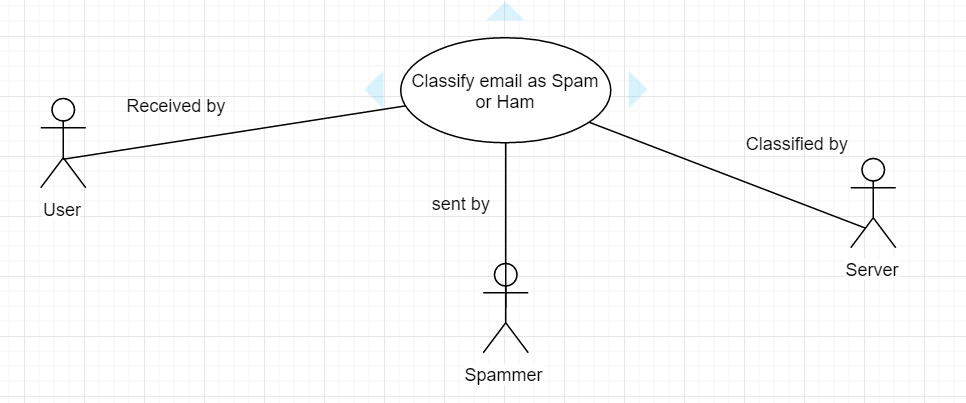
\includegraphics[width=1.0\linewidth]{usecase1.PNG}\caption{Use Case Diagram for the Spam Classification System}
\end{figure}


\subsection{SEQUENCE DIAGRAM}

The sequence of steps involved in spam classification is shown in the figure. The sequence diagram shown showcases the various functional classes in the system which perform various processes to process the data and develop the feature space/feature set. The features are then classified using a feed forward neural network.
\\
\begin{figure}[ht]
\centering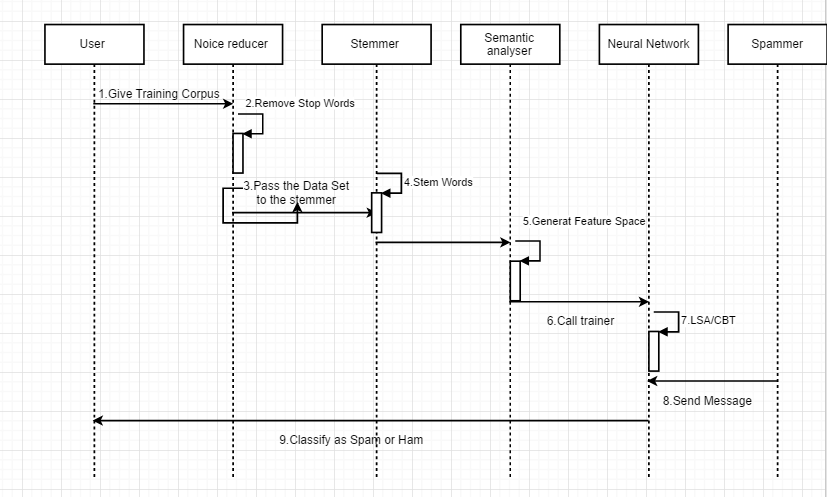
\includegraphics[width=0.82\linewidth]{sd.PNG}\caption{Sequence Diagram for the Spam Classification System}
\end{figure}


